\documentclass[11pt, oneside]{article}
\usepackage[a4paper,bindingoffset=0.2in,%
            left=1in,right=1in,top=1in,bottom=1in,%
            footskip=.25in]{geometry}
\usepackage{graphicx}
\usepackage{enumerate}
\usepackage{url}
\usepackage{hyperref}
\usepackage{pbox}
\usepackage{CJKutf8}
\usepackage{mathtools}
\usepackage{microtype}
\usepackage[htt]{hyphenat}
\renewcommand{\vec}[1]{\mathbf{#1}}


\begin{document}
\title{Assignment 1: Naive Bayes (II)}
\author{Xiyou Zhou, 13307130189 \\ Computer Science and Technology}
\maketitle
\section{Content}
\subsection{Modeling using Naive Bayes}
Here we are given such a problem: There is a email dataset split into training set of size $N$ and test set of size $M$. In training set, We have $D$ features represented as $\vec{X} \in R^D$ and the label $Y \in \{0, 1\}$ regarding whether this email is spam. In test set, we only have the same number of features for each instance and we would like to figure out the correct label for each instance.

Therefore, we can represent the probability of label $Y$ given the features $\vec{X}$ as $P(Y|\vec{X})$. Following the Bayes Rule:
$$
	P(Y|\vec{X}) = \frac{P(\vec{X}|Y)P(Y)}{P(\vec{X})} \propto P(\vec{X}|Y)P(Y) = P(Y)\prod_i P(X_i|Y)
$$
While we are given $X_i$ as continuous value and we can also preprocess the values as binary value. Consider word "purchase", the existence of such word in spam is very common and the existence rather than frequency of such word matters more in classification. That's why we can use binarized feature input can be used. Actually, our later experiments show Beta-Bernoulli Naive Bayes Classifier using binarized input performs well.

Here we only need to estimate $P(X_i|Y)$ given the training data. Consider if we use binarized features, the features can be each considered as results of several coin toss, where 1 regards the head and 0 regards the tail and estimate the probability $\theta$ of tossing head. The likelihood is $P(D|\theta) = \theta^{N_1} + \theta^{N_0}$. Here we can use Bernoulli distribution's conjugate prior distribution Beta Distribution as the prior since they have the same form. Thus, the prior is:
$$P(\theta) = Beta(\theta | \alpha, \beta) = \frac{\theta^{\alpha_1-1}+(1-\theta)^{\alpha_0-1}}{Beta(\alpha, \beta)}$$
Thus, the posterior is:
$$P(\theta|D) \propto \theta^{\alpha+N_1-1}+(1-\theta)^{\beta+N_0-1}$$
Therefore, the MAP of $\theta$ is $\frac{\alpha+N_1}{\alpha+\beta+N_1+N_0}$. We can estimate $P(X_i|Y)$ using the MAP.

When features given as continuous data, we can fit the distribution of such feature $X_i$ given label $Y$ to a Gaussian distribution and simply use the fitted mean and variance to predicate the probability density at given test data feature.

For model selection, here we use Beta-Bernoulli model according to their conjugation and the fact that binarized data make sense. Also, we select Gaussian Naive-Bayes model since we would like to predicate the probability density given feature input.

Here the assumption of i.i.d features results in we can derive $P(\vec{X}|Y)$ from $\prod_i P(X_i|Y)$. If not i.i.d we would have to figure out the dependence situation inside features and recalculate $P(\vec{X}|Y)$. In practice, we would assume i.i.d for Naive Bayes models and the result is not bad even if there are dependence in features.

\subsection{Preprocessing}

The binarization processing make it possible to use Beta-Bernoulli model to predicate the label since it turns continuous value into binary integer value. Also, according to our observation, the existence of words sometimes overweights their frequency. Therefore, binarization can be used for such model to reach great performance.

The log-transformation put extreme large and extreme small value into a reasonably common interval. Therefore later calculation won't be affected by extreme value.

The z-normalization-transformation turns the mean to 0 and the variance to 1. Therefore, the data is also put into a reasonably common interval for the whole dataset level.

\section{Beta-Bernoulli Naive Bayes}
Here we can observe the error rate change with $\alpha$ increases. The red line indicates training error and the green line indicates test error. Clearly, the error level increases as $\alpha$ increases for both training data and test data. When $\alpha = 1$, the training error is $11.25611\%$, test error is $11.00260\%$. When $\alpha = 10$, the training error is $11.97390\%$, test error is $11.19792\%$. When $\alpha = 100$, the training error is $13.99674\%$, test error is $13.28125\%$. To my surprise, the training error rate is higher than the test error rate, I guess it's because of the the data in two sets might be very uniform in feature distribution and the training set is bigger and contains more special data.

Also, when $\alpha$ increases the posterior is more affected by Beta Prior Distribution and thus makes worse performance since the prior is even for both sides.

\begin{figure}[h]
\centering
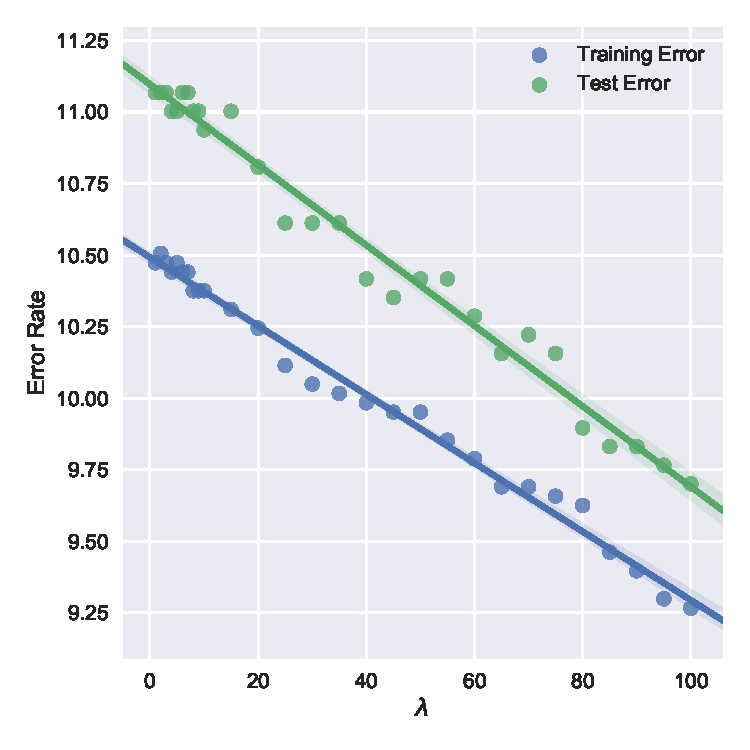
\includegraphics{foo.pdf}
\caption{Plot of Error Rate Change with $\alpha$}
\end{figure}

\section{Gaussian Naive Bayes}

It turns out $17.61827\%$ training error and $18.68490\%$ test error for non-preprocessing, $17.61827\%$ training error and $19.01042\%$ test error for z-normalization preprocessing, $16.34584\%$ training error and $18.09896\%$ test error for log preprocessing. Using sklean GaussianNB achieved similar results. I also tested with Random Forest Classifier and reached $6.18490\%$ test set error rate.
 
\begin{thebibliography}{9}
\bibitem{UBCMLNote8}
UBC Machine Learning CS540 Lecture Note 8,
\\\texttt{https://www.cs.ubc.ca/\~{}murphyk/Teaching/CS540-Fall08/L8.pdf}

\bibitem{lucius-yu}
Beta Distribution, Dirichlet Distribution and Bayesian Parameter Estimation,
\\\texttt{https://lucius-yu.github.io/docs/probability/BaysianEstimation/}

\end{thebibliography}

\end{document}